% k-NN vs linear scatter for ablation (fill @200 epoch when available).
% Preliminary @100 epoch points shown as hollow markers.
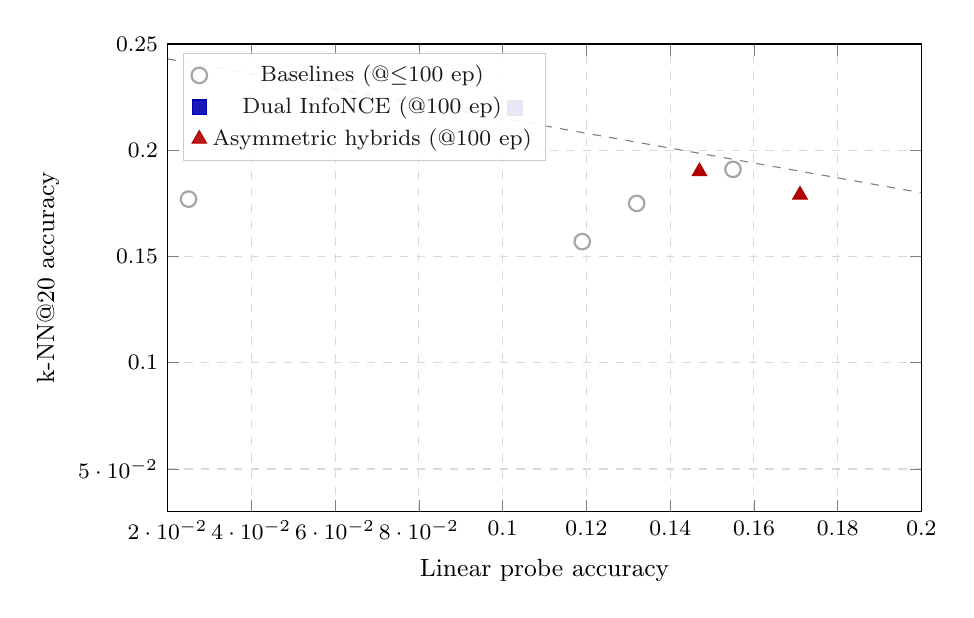
\begin{tikzpicture}
  \begin{axis}[
    width=0.92\linewidth,
    height=0.62\linewidth,
    xlabel={Linear probe accuracy},
    ylabel={k-NN@20 accuracy},
    xmin=0.02, xmax=0.20,
    ymin=0.03, ymax=0.25,
    grid=major,
    grid style={dashed,gray!30},
    legend style={
      at={(0.02,0.98)},
      anchor=north west,
      font=\footnotesize,
      fill=white,
      fill opacity=0.9,
      draw=gray!40,
    },
    tick label style={font=\footnotesize},
    label style={font=\small},
  ]
    % --- Published-style baselines (@100 ep, preliminary) ---
    \addplot[
      only marks,
      mark=*,
      mark size=2.8pt,
      color=gray!70,
      fill=white,
      thick,
    ] coordinates {
      (0.132, 0.175)  % EMA JEPA @100
      (0.155, 0.191)  % EMA JEPA peak @50
      (0.025, 0.177)  % Uniformity @90
      (0.119, 0.157)  % VICReg curriculum @10
    };
    \addlegendentry{Baselines (@${\leq}$100 ep)}

    % --- InfoNCE family (@100 ep) ---
    \addplot[
      only marks,
      mark=square*,
      mark size=2.6pt,
      color=blue!70!black,
    ] coordinates {
      (0.103, 0.220)  % Dual InfoNCE (~@90)
    };
    \addlegendentry{Dual InfoNCE (@100 ep)}

    % --- Proposed hybrids (@100 ep) ---
    \addplot[
      only marks,
      mark=triangle*,
      mark size=3pt,
      color=red!70!black,
    ] coordinates {
      (0.147, 0.190)  % MVC @30
      (0.171, 0.179)  % SIGReg hybrid @90-100
    };
    \addlegendentry{Asymmetric hybrids (@100 ep)}

    % --- @200 ep: update coordinates when sweep completes ---
    % \addplot[only marks, mark=star, ...] coordinates { (linear, knn) ... };

    % Visual guide: higher linear + higher k-NN is upper-right
    \addplot[gray, dashed, domain=0.02:0.20] {0.25 - 0.35*x};
  \end{axis}
\end{tikzpicture}
